\documentclass[11pt]{article}

\usepackage[utf8]{inputenc}
\usepackage[T1]{fontenc}
\usepackage[ngerman]{babel}
\usepackage{lmodern}
\usepackage[german=quotes]{csquotes}
\usepackage{amsmath}
\usepackage{amssymb}
\usepackage{amsthm}
\usepackage{graphicx}
\usepackage{scrpage2}
\usepackage{geometry}
\usepackage{tikz, tikz-3dplot}
\usepackage[bookmarks=true,
bookmarksopen=true,
bookmarksnumbered=false,
pdfstartpage=1,
baseurl=,
pdftitle={ },
pdfauthor={Pascal Gepperth},
pdfstartview={FitH},
pdfsubject={ },
pdfkeywords={ },
breaklinks=true,
colorlinks=true,
linkcolor=black,
anchorcolor=black,
citecolor=black,
filecolor=black,
menucolor=black,
pagecolor=black,
urlcolor=black ]{hyperref}
\newcommand{\de}{\mathrm{d}}
\newcommand{\dif}[1]{\frac{\mathrm{d}}{\mathrm{d}#1}}
\usepackage{enumerate}
\newcommand{\ray}[1]{\stackrel{\rightharpoonup}{#1}}
\usepackage{marginnote}
\let\marginpar\marginnote
\renewcommand*{\marginfont}{\footnotesize}
\usepackage{siunitx}

\usetikzlibrary{angles,quotes}
\newcommand{\cross}[1]{
\draw ($(#1) + (-.1,-.1)$) -- ($(#1) + (.1,.1)$);
\draw ($(#1) + (.1,-.1)$) -- ($(#1) + (-.1,.1)$);
}

\geometry{left=3cm, right=3cm, top=3cm, bottom=3cm}

\pagestyle{scrheadings}
\ohead{Pascal Gepperth}
\ifoot{\today}

\begin{document}

\section*{Sitzung 1}
\subsection*{Uni-Teil}
\subsubsection*{Erweiterung des ersten Strahlensatzes}
\begin{equation*}
\begin{aligned}
&& \frac{a}{c} &= \frac{a +b}{c + b}\\
\Leftrightarrow && \frac{c+d}{c} &= \frac{a+b}{a}\\
\Leftrightarrow && \frac{d}{c} &= \frac{b}{a}\\
\Leftrightarrow && \frac{a}{b} &= \frac{c}{d}
\end{aligned}
\end{equation*}
\subsubsection*{Zweiter Strahlensatz}
Es gilt der erste Strahlensatz.\\
\textbf{Skizze:}
\begin{center}
	\begin{tikzpicture}[scale = 2, thick]
		\coordinate (A) at (2,2);
		\coordinate (B) at (0,0);
		\coordinate (C) at (2,0);
		\coordinate (D) at (3,1);
		\coordinate (E) at (3,0);
		\coordinate (F) at (3,3);
		
		\draw (A)node[above]{$A$} -- (B)node[below]{$B$} -- (C)node[below]{$C$} -- (A) -- (F)node[above]{$F$} -- (E)node[below]{$E$} -- (C) -- (D)node[right]{$D$};
	\end{tikzpicture}
\end{center}
Es gilt mit dem ersten, erweiterten Strahlensatz und Zentrum $ B $
\begin{equation}
\begin{aligned}
\frac{BC}{CE} = \frac{BA}{AF} \label{eq:ZentrB}
\end{aligned}
\end{equation}
sowie für Zentrum $ E $
\begin{equation*}
\begin{aligned}
\frac{ED}{DF} = \frac{EC}{CB}
\end{aligned}
\end{equation*}
und somit natürlich auch
\begin{equation}
\begin{aligned}
\frac{DF}{ED} = \frac{BC}{CE} \label{eq:ZentrE}
\end{aligned}
\end{equation}
Aus (\ref{eq:ZentrB}) und (\ref{eq:ZentrE}) folgt dann
\begin{equation*}
\begin{aligned}
&&\frac{BA}{AF} &= \frac{DF}{ED}\\
\Leftrightarrow && \frac{BA}{DF} &= \frac{AF}{ED}
\end{aligned}
\end{equation*}
Da $ AF \parallel CD $ und $ AC \parallel DF $ ist $ ACDF $ ein Parallelogramm. Damit gilt $ AC = DF $ und folglich
\begin{equation*}
\begin{aligned}
&& \frac{BA}{DF} &= \frac{AF}{DE}\\
\Leftrightarrow && \frac{DE}{DF} &= \frac{AF}{BA}\\
\Leftrightarrow && \frac{DE}{DF} &= \frac{AF}{BA}\\
\Leftrightarrow && \frac{DE + DF}{DF} &= \frac{AF + BA}{BA}\\
\Leftrightarrow && \frac{BA}{DF} &= \frac{AF +BA}{DE + DF}\\
\Leftrightarrow && \frac{BA}{AC}&= \frac{BF}{EF}
\end{aligned}
\end{equation*}
\subsubsection*{Widerlegung der Umkehrung}
Betrachte die Punkte $ A(0,0), B(2,2), C(1,0), D(3,0) $.\\
\textbf{Skizze:}
\begin{center}
	\begin{tikzpicture}[scale = 2, thick]
		\coordinate (A) at (0,0);
		\coordinate (B) at (2,2);
		\coordinate (C) at (1,0);
		\coordinate (D) at (3,0);
		
		\draw (B)node[above]{$B$} -- (A)node[left]{$A$} -- (C)node[below]{$C$} -- (D)node[below]{$D$};
		\draw[dashed] (D) -- (B) -- (C);
	\end{tikzpicture}
\end{center}
Offenbar gilt
\begin{equation*}
\begin{aligned}
\frac{AB}{BC} &= \frac{AB}{BC},
\end{aligned}
\end{equation*}
doch die Geraden $ B\lor C $ und $ B \lor D $ sind verschieden, da $ C \neq D $, es gilt aber
\begin{equation*}
\begin{aligned}
B \in B\lor C \cap B\lor D \neq \emptyset.
\end{aligned}
\end{equation*}
Folglich sind die Geraden nicht parallel.
\newpage
\section*{Sitzung 2}
\subsection*{Schul-Teil}
\subsubsection*{Eigenschaften der Zentrischen Streckung (Elemente 5)}
Beispiele an Konstruktionen mit maßstäblicher Vergrößerung.
\paragraph{Definition}
Eine \textbf{zentrische Streckung} wird festgelegt durch das \textbf{Streckzentrum \textit{Z}} und den \textit{positiven} \textbf{Streckfaktor \textit{k}}.\\
Zu einem Punkt erhältst du den Bildpunkt wie folgt:
\begin{enumerate}[(1)]
	\item Wenn der Punkt $ P $ nicht mit dem Zentrum zusammenfällt, dann erhält man den Bildpunkt $ P' $ wie folgt:
	\begin{enumerate}[(a)]
		\item Zeichne die Halbgerade $ \ray{ZP} $.
		\item Zeichne den Punkt $ P' $ auf der Halbgeraden $ \ray{ZP} $ so, dass gilt
		\begin{align*}
		\left|ZP'\right| = k \cdot \left|ZP\right|
		\end{align*}
	\end{enumerate}
	\item Der Bildpunkt $ Z' $ von $ Z $ fällt mit $ Z $ zusammen: $ Z' = Z $.
\end{enumerate}
\paragraph{Zentrische Streckung mit negativem Streckfaktor}
Eingeführt als zentrische Streckung um $ \left|k\right| $ und anschließender Punktspiegelung in $ Z $.
\paragraph{Diskussion}
S.18, Afg 12
\paragraph{Eigenschaften}
Betrachtung verschiedener Abbildungen (vgl S.19) \marginpar{Abb. ungenau, nur intuitive Vermutungen}
\begin{enumerate}[(1)]
	\item Drehung + Verkleinerung
	\item Stauchung von Winkel
	\item Zentrische Streckung Dreieck
	\item Verschiedene Streckungsfaktoren
\end{enumerate}
mit Hinblick auf zentrische Streckungen. Beurteilung:
\begin{enumerate}[(1)]
 \item nicht, da $ AB $ nicht parallel zu $ A'B' $.
 \item nicht, da Winkel nicht erhalten.
 \item ja.
 \item nicht, da unterschiedliche Streckfaktoren.
 \end{enumerate}
\paragraph{Satz}
Für jede \textit{zentrische Streckung} mit einem positiven Streckfaktor $ k $ gilt:
\begin{enumerate}[(a)]
	\item Gerade und Bildgerade sind parallel.
	\item Bildstrecke ist k-mal so lang wie Originalstrecke.
	\item Winkel und Bildwinkel sind gleich groß.
\end{enumerate}
\paragraph{Beweis des Satzes}
\begin{enumerate}[(a)]
	\item Wird nicht bewiesen.
	\item Betrachtung zweier Fälle
	\begin{enumerate}[1.]
		\item Fall: Die Strecke $ AB $ liegt auf einer Geraden durch das Streckzentrum. \marginpar{$ Z \in A\lor B $}\\
		Dann gilt
		\begin{equation*}
		\begin{aligned}
		\left|ZA'\right| = k \cdot \left|ZA\right| \qquad \text{und} \qquad \left|ZB'\right| = k\cdot \left|ZB\right|.
		\end{aligned}
		\end{equation*}
		Ohne Einschränkung ist
		\begin{equation*}
		\begin{aligned}
		\left|ZA\right| < \left|ZB\right|.
		\end{aligned}
		\end{equation*}
		Dann gilt \textit{(\enquote{Aus der Zeichnung entnehmen wir:})}
		\begin{center}
			\begin{tikzpicture}
			\coordinate (Z) at (0,0);
			\coordinate (A) at (1.5,0);
			\coordinate (B) at (2.5,0);
			\coordinate (A') at (3,0);
			\coordinate (B') at (5,0);
			
			\draw (Z) node[anchor=north]{$Z$} -- (A) node[below]{$A$} -- (B) node[below]{$B$} -- (A') node[below]{$A'$} -- (B') node[below]{$B'$};
			\cross{Z};
			\cross{A};
			\cross{B};
			\cross{A'};
			\cross{B'};
			\end{tikzpicture}
		\end{center}
		\begin{equation*}
		\begin{aligned}
		\left|AB\right| = \left|ZB\right| - \left|ZA\right| \qquad \text{und} \qquad \left|A'B'\right| = \left|ZB'\right| - \left|ZA'\right|.
		\end{aligned}
		\end{equation*}
		Infolge dessen gilt
		\begin{equation*}
		\begin{aligned}
		\left|A'B'\right| &= \left|ZB'\right| - \left|ZA'\right|\\
		&= k \cdot\left|ZB\right| - k \cdot \left|ZA\right|\\
		&=k \cdot \left(\left|ZB\right| - \left|ZA\right|\right)\\
		&= k \left|AB\right|
		\end{aligned}
		\end{equation*}
		\item Fall: Die Strecke $ AB $ liegt nicht auf einer Geraden durch das Streckzentrum. \marginpar{$ Z \notin A\lor B $}\\
		\begin{center}
			\begin{tikzpicture}[thick,yscale = 1.8]
				\coordinate (Z) at (0,0);
				\coordinate (A) at (2,1);
				\coordinate (A') at ($1.5*(A)$);
				\coordinate (B) at (3,0);
				\coordinate (B') at ($1.5*(B)$);
				\coordinate (C) at ($(A)-(B)$);
				\coordinate (C') at ($(A')-(B')$);
				
				\draw (Z) node[anchor=north]{$ Z $} -- (A) node[anchor=south east]{$ A $} --(A') node[anchor=south east]{$ A' $} -- ($(A') + (A)$);
				\draw (Z) -- (B) node[anchor=north]{$ B $} -- (B') node[anchor=north]{$ B' $} -- ($(B') + (B)$);
				\draw (Z) -- (C) node[anchor=north east]{$ C $} -- (C') node[anchor=north east]{$ C' $} -- ($(C') + (C)$);
				\draw (C) -- (A) -- (B);
				\draw (C') -- (A') -- (B');
				
				\node at ($(C') + 0.5*(C)$) [anchor= south west]{$ g $};
			\end{tikzpicture}
		\end{center}
	Betrachte Parallele $ g $ zu $ AB $ durch $ Z $. Dann ist $ g $ nach (a) auch parallel zu $ A'B' $, da
	\begin{equation*}
	\begin{aligned}
	AB \parallel A'B'.
	\end{aligned}
	\end{equation*}
	Strecken $ AB $ und $ A'B' $ werden auf $ g $ abgetragen (Schnitt von $ g $ und Parallele von $ ZB $ durch $ A $ bzw. $A'$).
	Damit sind $ ZBAC $ und $ ZB'A'C' $ Parallelogramme und es gilt
	\begin{equation*}
	\begin{aligned}
	\left|ZC\right| &= \left|AB\right|\\
	\left|ZC'\right| &= \left|A'B'\right|.
	\end{aligned}
	\end{equation*}
	Nun ist $ C' $ auch Bildpunkt von $ C $, da nach (a) $ C'A' $ die Bildgerade von $ CA $ ist. Damit gilt
	\begin{equation*}
	\begin{aligned}
	\left|A'B'\right| &= \left|ZC'\right|\\
	&= k \left|ZC\right|\\
	&= k \left|AB\right|
	\end{aligned}
	\end{equation*}
	\end{enumerate}
	\item Sei $ \alpha' $ der Bildwinkel von $ \alpha $ nach zentrischer Streckung in Zentrum $ Z $.
	\begin{center}
		\begin{tikzpicture}[thick]
			\coordinate (Z) at (0,0);
			\coordinate (A) at (1,.2);
			\coordinate (A') at ($3*(A)$);
			\coordinate (B) at ($(A) + (1,-3)$);
			\coordinate (B') at ($(B) - (A) + (A')$);
			\coordinate (C) at ($(A) + (3,-3)$);
			\coordinate (C') at ($(C) - (A) + (A')$);
			\coordinate (A'') at ($1.5*(A')$);
			
			\draw (Z) node[left]{$Z$} -- (A'');
			\cross{Z};
			\draw (A) node[above]{$A$} -- (C);
			\draw (A) -- (B);
			
			\draw (A') node[above]{$A'$} -- (C');
			\draw (A') -- (B');
			
			\pic [draw, angle radius = 1cm] {angle = B--A--C};
			\pic [draw, angle radius = 0.7cm] {angle = C--A--A'};
			\pic [draw, angle radius = 1.3cm] {angle = B--A--A'};
			\pic [draw, angle radius = 1cm] {angle = B'--A'--C'};
			\pic [draw, angle radius = 0.7cm] {angle = C'--A'--A''};
			\pic [draw, angle radius = 1.3cm] {angle = B'--A'--A''};
			
			\node at ($(A) + (.4,-.15)$) {$\beta$};
			\node at ($(A') + (.45,-.15)$) {$\beta'$};
			
			\node at ($(A) + (.4,-.65)$) {$\alpha$};
			\node at ($(A') + (.4,-.65)$) {$\alpha'$};
			
			\node at ($(A) + (0.9,-.40)$) {$\gamma$};
			\node at ($(A') + (0.9,-.35)$) {$\gamma'$};
		\end{tikzpicture}
	\end{center}
	Nach (a) sind die Schenkel an $ A $ bzw. $ A' $ paarweise zueinander parallel.\\
	Mit dem Stufenwinkelsatz gilt dann
	\begin{equation*}
	\begin{aligned}
	\beta &= \beta'\\
	\gamma &= \gamma'
	\end{aligned}
	\end{equation*}
	sowie
	\begin{equation*}
	\begin{aligned}
	\alpha &= \gamma - \beta\\
	\alpha' &= \gamma' - \beta'
	\end{aligned}
	\end{equation*}
	und folglich
	\begin{equation*}
	\begin{aligned}
	\alpha' &= \gamma' - \beta'\\
	&= \gamma - \beta\\
	&= \alpha
	\end{aligned}
	\end{equation*}
\end{enumerate}
\begin{flushright}
	$ \Box $
\end{flushright}
\subsubsection*{Vergleich der Schulbücher}
\paragraph{BUCHTITEL 1}
\begin{itemize}
	\item Beginn mit \enquote{maßstäblicher Vergrößerung}.
	\begin{itemize}
		\item Streckenverhältnis von Original- zu Bildstrecke bleibt gleich
		\begin{equation*}
		\begin{aligned}
		k = \frac{a'}{a} = \frac{b'}{b}
		\end{aligned}
		\end{equation*}
		\item (Bild-)Winkel sind gleich weit.
	\end{itemize}
	\item zentrische Streckung als \enquote{Abbildung} mit Streckzentrum $ Z $ und Streckfaktor $ k $, sodass jedem Punkt $ P $, der nicht das Zentrum ist, ein Punkt $ P' $ zugeordnet wird und
	\begin{itemize}
		\item $ P' $ liegt auf dem Strahl $ \ray{ZP} $
		\item \begin{equation*}
		\begin{aligned}
		\overline{ZP'} = k \cdot \overline{ZP}
		\end{aligned}
		\end{equation*}
	\end{itemize}
	\item Vorerst $ k > 0 $
	\item \enquote{Satz von der zentrischen Streckung}, sodass Geraden auf parallele Geraden abgebildet werden
	\item Mit dem Satz begründen sich Winkeltreue und Teilverhältnistreue
	\item Bsp. zum konstruieren einer zentr. Streck.
	\item Bsp. Streckzentrum bestimmen
	\item Üb. Entscheiden ob zentr. Streck.
\end{itemize}
\paragraph{Lambacher Schweizer}
\begin{itemize}
	\item Zentrische Streckung als reine Konstruktionsanleitung. \marginpar{Mache dies, dann das}
	\item Bsp. Konstruktion
	\item Bsp. Zentrum finden
\end{itemize}
\paragraph{Delta}
\begin{itemize}
	\item Einführung über Vergrößerung und Verkleinerung
	\begin{itemize}
		\item intuitiv und anschaulich
		\item Anschauliche Beispiele (praktisch durchführbar)
		\item Wertetabelle
		\begin{center}
			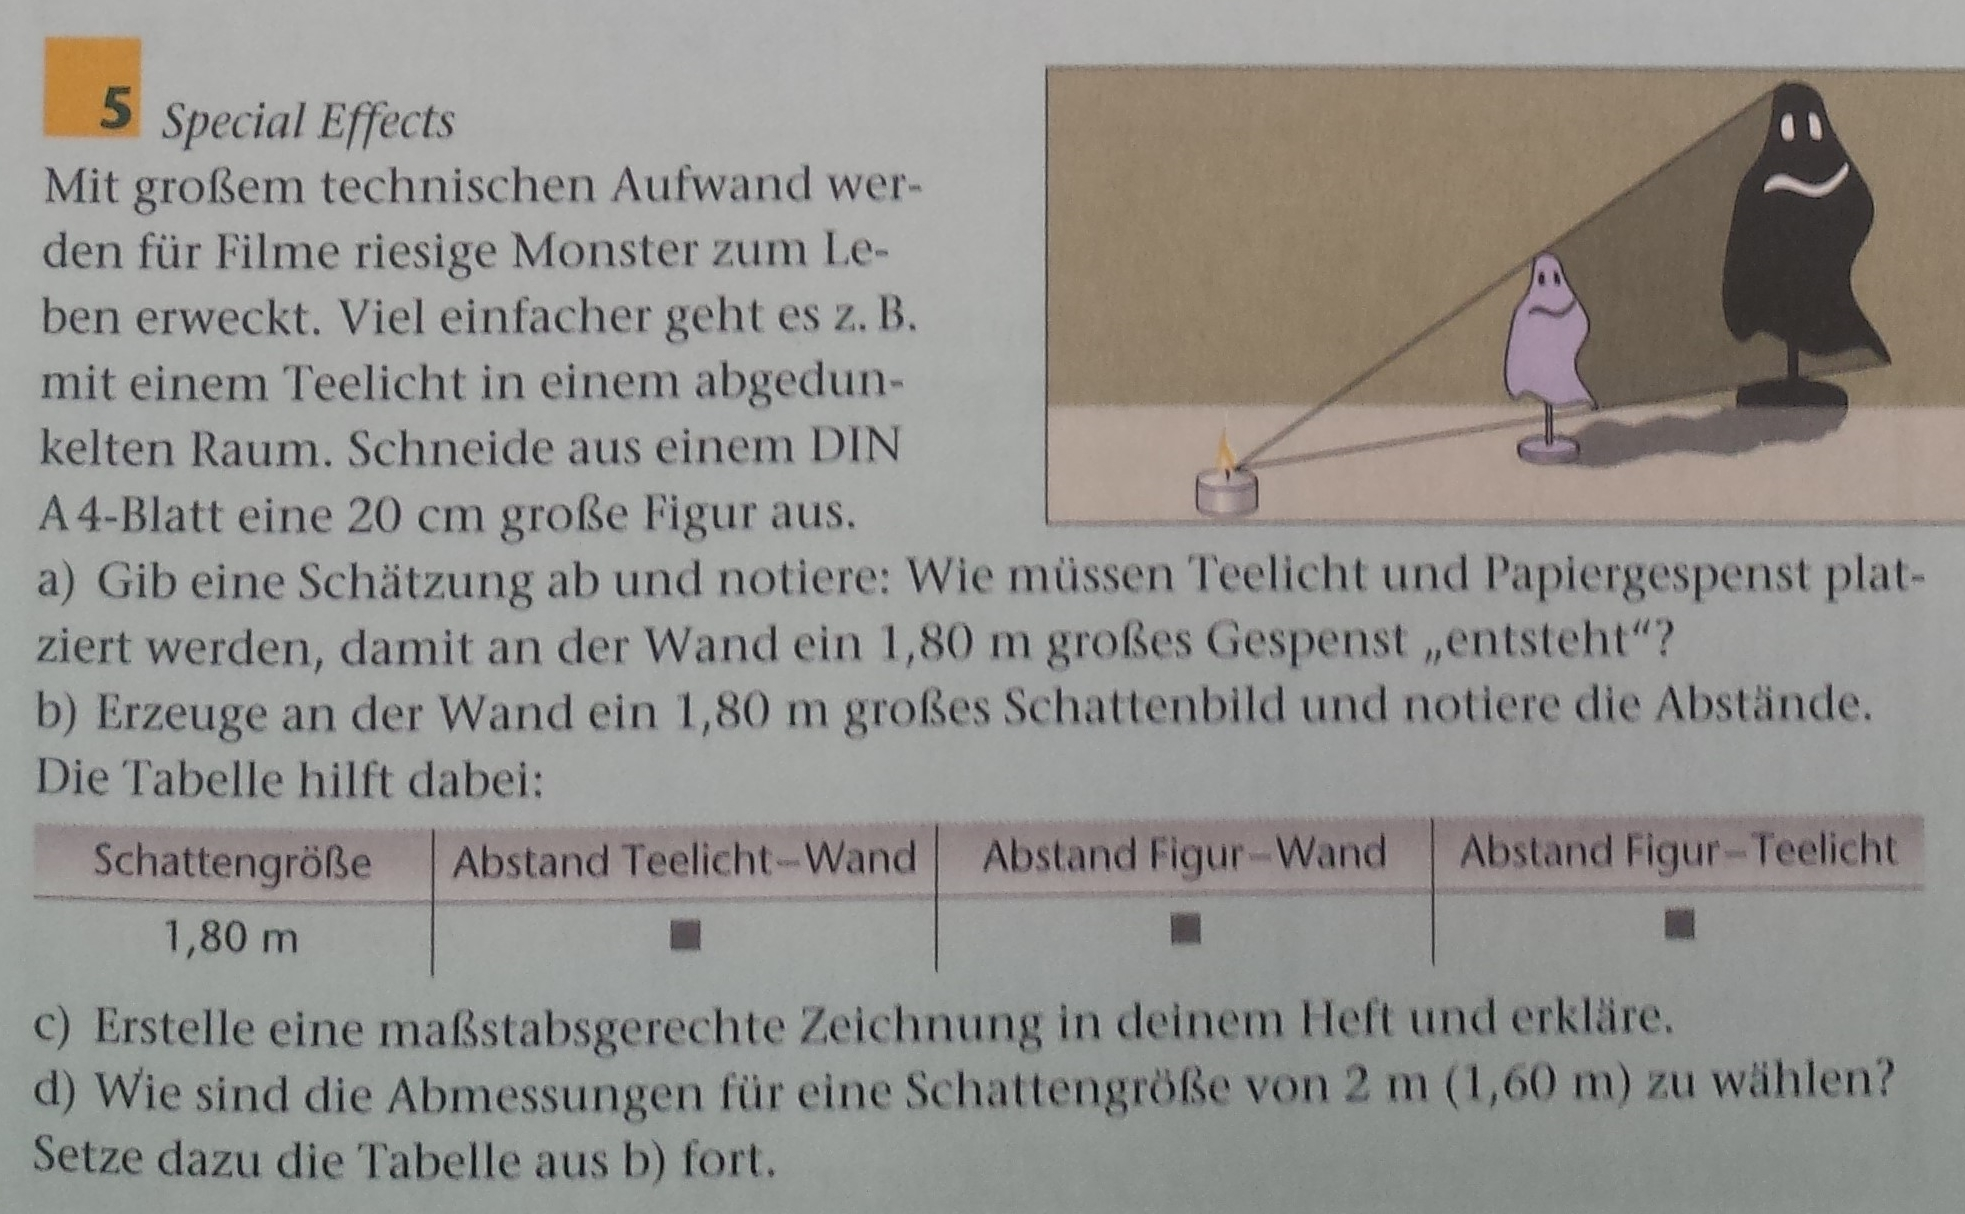
\includegraphics[width=0.7\linewidth]{ZS_Bsp}
		\end{center}
	\end{itemize}
	\item Definition via Konstruktion (nur Bilder)
	\item Eigenschaften
	\begin{itemize}
		\item $ P' \in Z \lor P $
		\item $ \overline{ZA'} = k \cdot \overline{ZA} $
		\item $ \alpha = \alpha' $
		\item $ BC \parallel B'C' $
	\end{itemize}
	\item negatives $ k $ extra behandelt (Bsp Lochkamera)
	\item Übungsaufgabe: Erkenne ob ZS
	\item Übungsaufgabe: Nicht erkennbar, was Ausgangs- und Bildfigur (interpretativ)
\end{itemize}
\end{document}

